\documentclass[a4paper,12pt]{article} % тип документа

% Поля страниц
\usepackage[left=2.5cm,right=2.5cm,
top=2cm,bottom=2cm,bindingoffset=0cm]{geometry}

% Пакет дял таблиц   
\usepackage{multirow} 

% Отступ после заголовка    
\usepackage{indentfirst}


% Рисунки
\usepackage{floatrow,graphicx,calc}
\usepackage{wrapfig}

%%% Работа с картинками
\usepackage{graphicx}  % Для вставки рисунков
\graphicspath{{images/}{images2/}}  % папки с картинками
\setlength\fboxsep{3pt} % Отступ рамки \fbox{} от рисунка
\setlength\fboxrule{1pt} % Толщина линий рамки \fbox{}
\usepackage{wrapfig} % Обтекание рисунков и таблиц текстом

% Создаёем новый разделитель
\DeclareFloatSeparators{mysep}{\hspace{1cm}}

% Ссылки?
\usepackage{hyperref}
\usepackage[rgb]{xcolor}
\hypersetup{				% Гиперссылки
  colorlinks=true,       	% false: ссылки в рамках
  urlcolor=blue          % на URL
}


% Русский язык
\usepackage[T2A]{fontenc}			% кодировка
\usepackage[utf8]{inputenc}			% кодировка исходного текста
\usepackage[english,russian]{babel}	% локализация и переносы




% Математика
\usepackage{amsmath,amsfonts,amssymb,amsthm,mathtools}

%%% Дополнительная работа с математикой
\usepackage{amsmath,amsfonts,amssymb,amsthm,mathtools} % AMS
\usepackage{icomma} % "Умная" запятая: $0,2$ --- число, $0, 2$ --- перечисление


% Что-то 
\usepackage{wasysym}


\begin{document}
\begin{center}
  \footnotesize{ФЕДЕРАЛЬНОЕ ГОСУДАРСТВЕННОЕ АВТОНОМНОЕ ОБРАЗОВАТЕЛЬНОЕ 			УЧРЕЖДЕНИЕ ВЫСШЕГО ОБРАЗОВАНИЯ}\\
  \footnotesize{МОСКОВСКИЙ ФИЗИКО-ТЕХНИЧЕСКИЙ ИНСТИТУТ\\(НАЦИОНАЛЬНЫЙ 			ИССЛЕДОВАТЕЛЬСКИЙ УНИВЕРСИТЕТ)}\\
  \hfill \break
  \hfill \break
  \hfill \break
  \hfill \break
\end{center}

\hfill \break
\hfill \break
\hfill \break
\hfill \break
\hfill \break
\hfill \break
\hfill \break
\hfill \break


\begin{center}   
  \hfill \break
  \hfill \break
  \hfill \break
  \large{Лабораторная работа № 3.1.1\\ \hfill \break\Large{Магнитометр}}\\
  \hfill \break
  \hfill \break
  \hfill \break
  \hfill \break
  \begin{flushright}
    Сирый Р.А.\\
    Б02-206
  \end{flushright}
  \hfill \break
  \hfill \break
  \hfill \break
\end{center}
\hfill \break
\hfill \break
\hfill \break
\hfill \break
\begin{center}
  Долгопрудный, 2023 г.
\end{center}
\thispagestyle{empty}

\newpage

\textbf{Цель работы:} определить горизонтальную составляющую магнитного
поля Земли и установить количественное соотношение между единицами
электрического тока в системах СИ и СГС.

\textbf{В работе используются:} магнитометр, осветитель со шкалой, источник питания, вольтметр, электромагнитный переключатель, конденсатор, намагниченный стержень, прибор для определения, периода крутильных колебаний, секундомер, рулетка, штангенциркуль.

\section{Теоретические сведения}

\subsection{Определение горизонтальной составляющей магнитного поля Земли}

\begin{figure}[H]
  \centering
  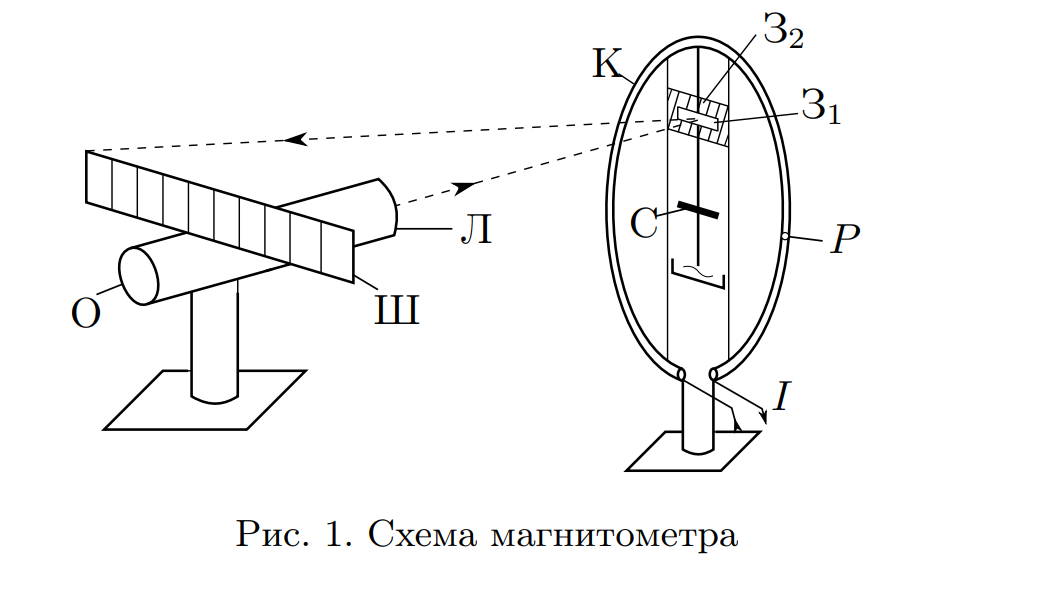
\includegraphics[scale=0.7]{1.png}
  \label{tc}
\end{figure}

Магнитометр (рис. 1) состоит из нескольких последовательно соединённых круговых витков К, расположенных вертикально. В центре кольца К радиусом R на тонкой неупругой вертикальной нити подвешена короткая магнитная стрелка С. Жёстко связанная со стрелкой крыльчатка
погружена в масло и служит для демпфирования колебаний.


\begin{figure}[H]
  \centering
  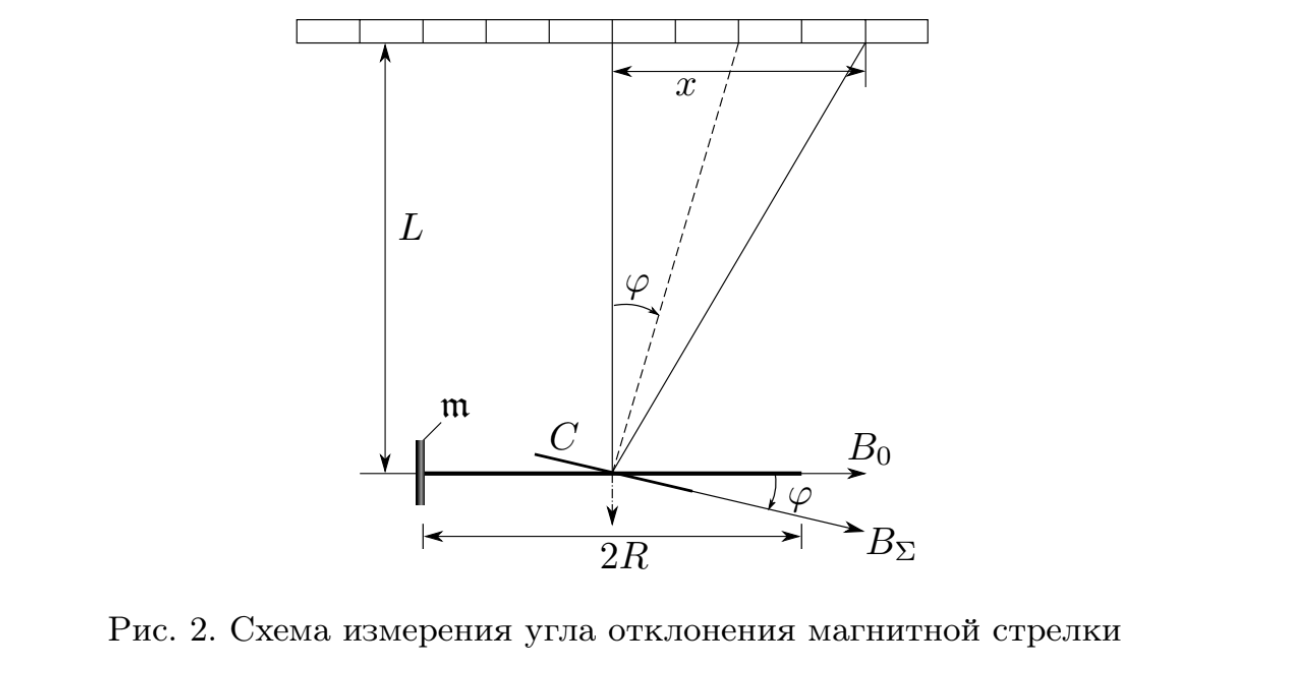
\includegraphics[scale=0.7]{2.png}
  \label{tc}
\end{figure}

В отсутствие других магнитных полей стрелка располагается по на-
правлению горизонтальной составляющей земного магнитного поля $B_{0}$ ,т. е. лежит в плоскости магнитного меридиана.
Прибор настраивают с помощью световых зайчиков, отражённых от
двух зеркал: З1, прикреплённого к стрелке (подвижный зайчик), и З2, расположенного в плоскости кольца К и жёстко связанного с ним (непо-
движный зайчик). Оба зеркала освещаются одним и тем же осветителем О. Вращением кольца вокруг вертикальной оси можно совместить оба зайчика. При этом плоскость витков совпадает с плоскостью магнитного меридиана.

При появлении дополнительного горизонтального магнитного поля  стрелка C установится по равнодействующей обоих полей (рис.2). В нашей установке дополнительное поле может быть создано
либо малым ферромагнитным стержнем, расположенным на кольце на
его горизонтальном диаметре ($B_{1}$), либо током, проходящим по кольцу
($B_{2}$). В обоих случаях дополнительное поле можно считать однородным,
так как размеры стрелки много меньше радиуса кольца.

Поле намагниченного стержня вдали от него может быть приближён-
но вычислено как поле точечного диполя:

\begin{equation}
  \mathcal{B(\mathbf{r})} = \frac{\mu_{0}}{4\pi}\cdot \left (3 \frac {\mathbf{m} \mathbf{r}}{r^5} - \frac{\mathbf{m}}{r^3} \right),
\end{equation}

где $\mathbf{m}$ — магнитный момент стержня, $\mathbf{r}$ — радиус-вектор, проведённый из центра диполя в точку наблюдения. На оси, перпендикулярной стержню, имеем

\begin{equation}
  B_{1}=\frac{\mu_{0}}{4\pi}\cdot \frac{\mathbf{m}}{R^3},
\end{equation}

где $R$ - радиус кольца.

Магнитное поле в центре кольца с током $I$ по закону Био и Савара
равно

\begin{equation}
  B_{1}=\frac{\mu_{0} I}{2\pi}N.
\end{equation}

Здесь $N$ - число витков в кольце, I - сила тока в амперах.

Так, поля $B_{0}$ и $B_{\perp}$ связаны соотношением 

\begin{equation}
  B_{\perp}=B_{0}\tan(\phi_{1}),
\end{equation}


где $\tan(\phi_{1}) = x_{1}/(2L)$ - тангенс угла отклонения стрелки.


Для исключения магнитного момента предлагается измерить период крутильных колебаний стержня в поле Земли. Подвешенный горизонтально за середину на тонкой длинной нити стержень в положении равновесия установится по полю Земли (упругость нити пренебрежимо мала). Период крутильных колебаний будет равен


\begin{equation}
  T = 2\pi\sqrt{\frac{J}{\mathbf{m}B_{0}}}
\end{equation}

Момент инерции стержня:

\begin{equation}
  J = m\left(\frac{l^2}{12}+\frac{r^2}{4}\right),
\end{equation}

где $m$ - масса стержня, $l$ - его длина, $r$ - его радиус.

Из вышеприведённых формул моно получить 

\begin{equation}
  B_{0} = \frac{2\pi}{TR}\sqrt{\frac{\mu_{0}JL}{2\pi Rx_{1}}}
\end{equation}


\subsection{Определение электродинамической постоянной}

Пропуская некоторый ток через витки магнитометра, по тангенсу угла отклонения стрелки $\tan(\varphi 2) = x_{2}/(2L)$ и по формулам (2) и (3) найдём силу тока в единицах СИ:

\begin{equation}
  B_{0} = \frac{2B_{0}R\tan(\phi_2)}{\mu_{0}R}.
\end{equation}

\begin{figure}[H]
  \centering
  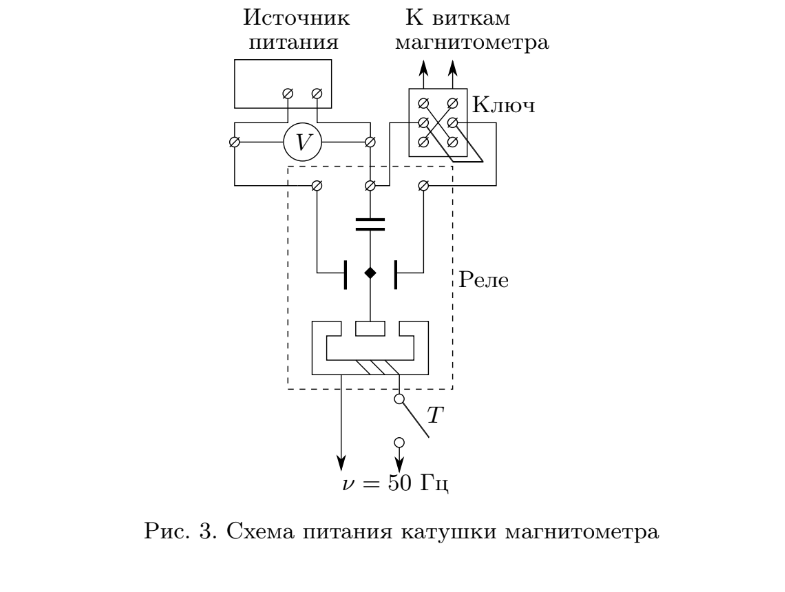
\includegraphics[scale=0.7]{3.png}
  \label{tc}
\end{figure}




Тот же ток можно измерить абсолютным образом по прошедшему в единицу времени заряду, что соответствует определению эталона тока в гауссовой системе (СГС). Если разрядить конденсатор известной ёмкости C, заряженный до напряжения U, через витки, то через них протечёт заряд $q = CU$ (рис. 3). Если $\nu$ раз в секунду последовательно заряжать конденсатор от источника и разряжать через витки, то через них за секунду протечёт заряд $CU\nu$. Средний ток, прошедший через витки, равен при этом

\begin{equation}
  I = CU\nu
\end{equation}


Итак, для вычисления абсолютного значения тока по (9) необходимо измерить напряжение U на конденсаторе известной ёмкости C. Напряжение необходимо выразить в единицах СГС (измерительные приборы, как правило, проградуированы в единицах СИ: 1 В = 1/300 ед. СГС).
Ёмкость конденсатора C [см] должна быть выражена в сантиметрах (1 Ф $\approx 9\cdot 10^{11}$ см).

По отношению численных значений одного и того же тока, выраженных в единицах СИ и СГС (гауссовой) по формулам (8) и (9) соответственно, можно определить значение электродинамической постоянной:

\begin{equation}
  c  = \frac{1}{10} \frac{I_{СГС}}{I_{СИ}}
\end{equation}


\section{Ход работы}

\subsection{Измерение горизонтальной составляющей магнитного поля Земли}

\begin{enumerate}
\item Включим осветитель и вставим в отверстие Р на горизонтальном диаметре кольца намагниченный стержень. Зафиксируем отклонение зайчика в одну сторону. Поменяв ориентацию стержня, зафиксируем отклонение в другую сторону. Оба значения оказались равными $x_{1} = 5,0\pm0,1$ см
\item Измерим расстояние $L$ от зеркала до шкалы и диаметр $D$ магнитометра:
  $$L = (112\pm1) \text{ см};\quad D = (40\pm1) \text{ см};\quad R = (20\pm0,5) \text{ см}$$
\item Подвесим стержень и опустим его в стеклянный сосуд, чтобы избежать влияния порывов воздуха. Добьёмся того, чтобы стержень совершал исключительно крутильные колебания.
  С помощью секундометра измерим время $k = 30$ колебаний и вычислим период одного колебания:
  \begin{equation*}
    t_{0} = (264,0\pm0,2)\text{ c} ;\quad T = \frac{t_{0}}{k} ;\quad T =(8,800\pm0,007)\text{ c}.
  \end{equation*}
\item Измерим с помощью штангенциркуля линейные размеры стержня:

  \begin{equation*}
    l = (40,00\pm0,02) \text{ см} ;\quad (d = 4,92\pm0,02) \text{ мм}
  \end{equation*}

  Здесь $d$ - диаметр стержня.

  По последним данным найдём момент инерции $J$ стержня:

  \begin{equation*}
    m = (5,900\pm0,001) \text{ гр} 
  \end{equation*}

  \begin{equation*}   
    J = (7,95 \pm 0,08) \cdot 10^{-7} \text{ }кгм^2
  \end{equation*}    

  
\item По формуле (7) найдём
  
  \begin{equation*}
    B_{0} = (1,51\pm0,07)\cdot10^{-5}\text{ Тл}
  \end{equation*}


  \subsection{Измерение электродинаминамической постоянной}

  \begin{enumerate}
  \item Уберём намагниченный стержень из гнезда магнитометра и соберём электическую схему, изображённую на рис.3; включим в сеть источник; замкнув ключ, подключим к цепи витки магнитометра.
  \item Измерим напряжение на конденсаторе $U$ и отклонение $x_{2}$ зайчика на шкале:
    \begin{equation*}
      U = (88\pm 1)\text{ В};\quad x_{21} = (11,3\pm0,1)\text{ см}
    \end{equation*}
    Поменяем полярность с помощью ключа:
    \begin{equation*}
      U = (88\pm1)\text{ В};\quad x_{22} = 11,0\pm0,1\text{см}
    \end{equation*}
    
    Среднее значение отклонения: $x_{2} = (11,2\pm0,1) \text{ см} $ 

  \item Характеристики приборов:
    $$N = 44,\quad C = (9,0\pm0,2)\cdot10^{5}\text{ см},\quad \nu = 50\text{ Гц} $$

  \item  По формулам (8) и (9) рассчитаем силы тока и электромагнитную постоянную:

    $$I = (5\pm1)\cdot10^{-3}\text{ ед. СИ} = (1,3\pm0,1)\cdot10^{7}\text{ ед. СГС}$$

    Итак,

    $$c = (2.6\pm0.5)\cdot10^{8} \text{ м/c}$$

    
  \end{enumerate}

  
\end{enumerate}






\section{Вывод и обсуждение результатов}

\begin{enumerate}
\item Полученное значение горизонтальной составляющей магнитного поля Земли сильно отличается от справочного значения ($B_{0} = 5\cdot10^{-4}$ Тл (по данным rusmagnet.ru) на порядок. Такое сильное расхождение может быть объяснено наличием влияющих на магнитное поле металлических предметов, таких как каркас здания, осветительная лампа, провода и так далее.
\item Полученное нами значение электродинамической постоянной отличается от истинного значения ($c = 2.99\cdot10^{8} $ м/c) примерно на 13\%. C учётом больших погрешностей определяемых выше величин данный результат можно считать удовлетворительным.
\end{enumerate}
\end{document}





